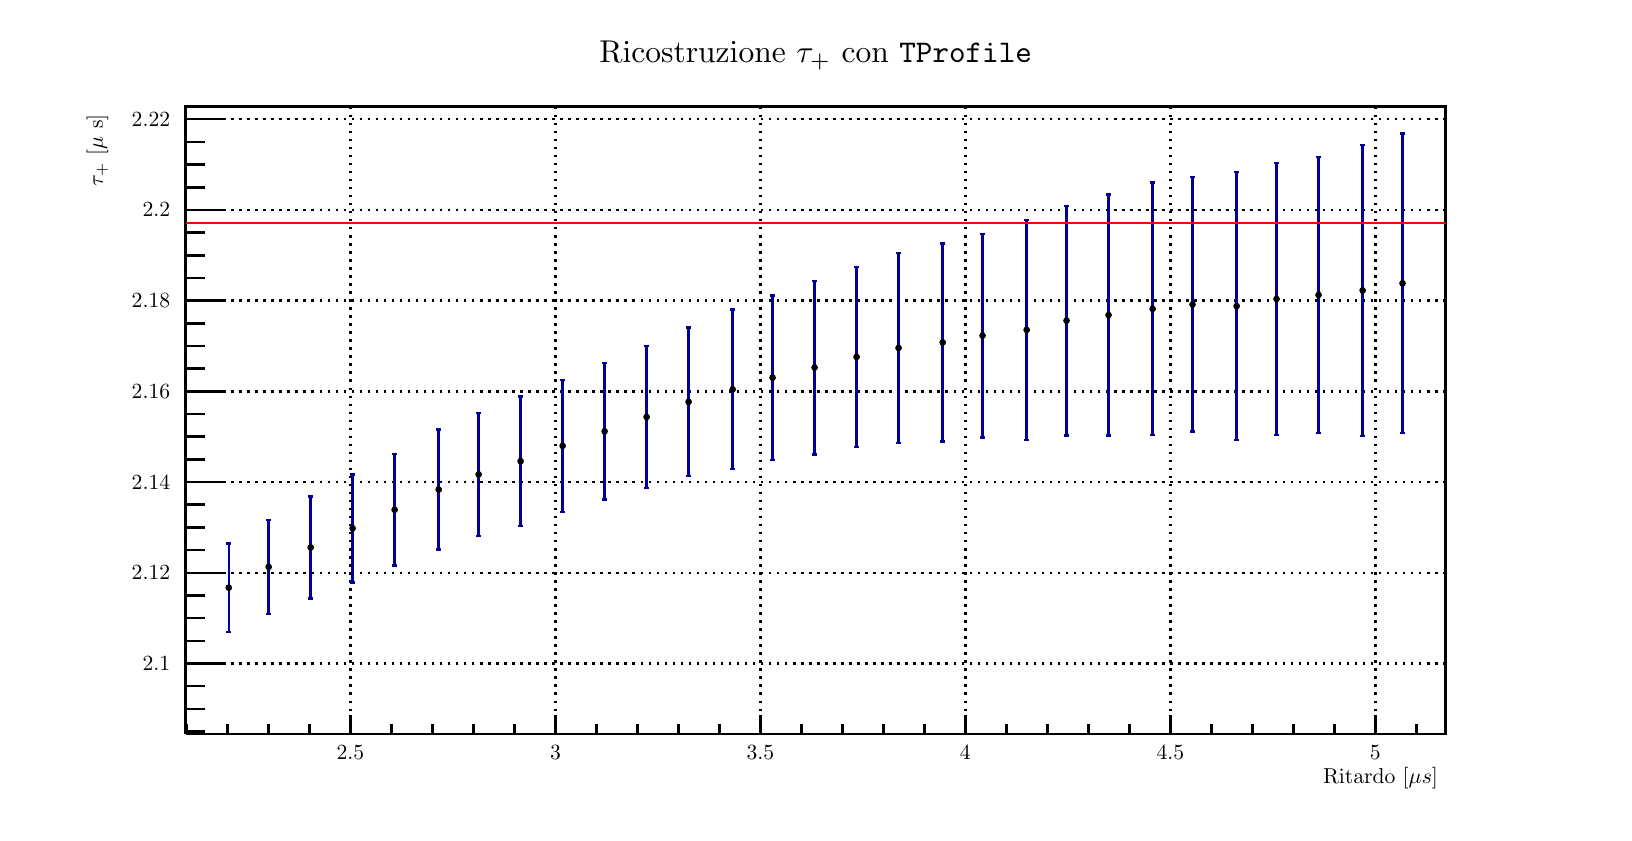
\begin{tikzpicture}
\pgfdeclareplotmark{cross} {
\pgfpathmoveto{\pgfpoint{-0.3\pgfplotmarksize}{\pgfplotmarksize}}
\pgfpathlineto{\pgfpoint{+0.3\pgfplotmarksize}{\pgfplotmarksize}}
\pgfpathlineto{\pgfpoint{+0.3\pgfplotmarksize}{0.3\pgfplotmarksize}}
\pgfpathlineto{\pgfpoint{+1\pgfplotmarksize}{0.3\pgfplotmarksize}}
\pgfpathlineto{\pgfpoint{+1\pgfplotmarksize}{-0.3\pgfplotmarksize}}
\pgfpathlineto{\pgfpoint{+0.3\pgfplotmarksize}{-0.3\pgfplotmarksize}}
\pgfpathlineto{\pgfpoint{+0.3\pgfplotmarksize}{-1.\pgfplotmarksize}}
\pgfpathlineto{\pgfpoint{-0.3\pgfplotmarksize}{-1.\pgfplotmarksize}}
\pgfpathlineto{\pgfpoint{-0.3\pgfplotmarksize}{-0.3\pgfplotmarksize}}
\pgfpathlineto{\pgfpoint{-1.\pgfplotmarksize}{-0.3\pgfplotmarksize}}
\pgfpathlineto{\pgfpoint{-1.\pgfplotmarksize}{0.3\pgfplotmarksize}}
\pgfpathlineto{\pgfpoint{-0.3\pgfplotmarksize}{0.3\pgfplotmarksize}}
\pgfpathclose
\pgfusepathqstroke
}
\pgfdeclareplotmark{cross*} {
\pgfpathmoveto{\pgfpoint{-0.3\pgfplotmarksize}{\pgfplotmarksize}}
\pgfpathlineto{\pgfpoint{+0.3\pgfplotmarksize}{\pgfplotmarksize}}
\pgfpathlineto{\pgfpoint{+0.3\pgfplotmarksize}{0.3\pgfplotmarksize}}
\pgfpathlineto{\pgfpoint{+1\pgfplotmarksize}{0.3\pgfplotmarksize}}
\pgfpathlineto{\pgfpoint{+1\pgfplotmarksize}{-0.3\pgfplotmarksize}}
\pgfpathlineto{\pgfpoint{+0.3\pgfplotmarksize}{-0.3\pgfplotmarksize}}
\pgfpathlineto{\pgfpoint{+0.3\pgfplotmarksize}{-1.\pgfplotmarksize}}
\pgfpathlineto{\pgfpoint{-0.3\pgfplotmarksize}{-1.\pgfplotmarksize}}
\pgfpathlineto{\pgfpoint{-0.3\pgfplotmarksize}{-0.3\pgfplotmarksize}}
\pgfpathlineto{\pgfpoint{-1.\pgfplotmarksize}{-0.3\pgfplotmarksize}}
\pgfpathlineto{\pgfpoint{-1.\pgfplotmarksize}{0.3\pgfplotmarksize}}
\pgfpathlineto{\pgfpoint{-0.3\pgfplotmarksize}{0.3\pgfplotmarksize}}
\pgfpathclose
\pgfusepathqfillstroke
}
\pgfdeclareplotmark{newstar} {
\pgfpathmoveto{\pgfqpoint{0pt}{\pgfplotmarksize}}
\pgfpathlineto{\pgfqpointpolar{44}{0.5\pgfplotmarksize}}
\pgfpathlineto{\pgfqpointpolar{18}{\pgfplotmarksize}}
\pgfpathlineto{\pgfqpointpolar{-20}{0.5\pgfplotmarksize}}
\pgfpathlineto{\pgfqpointpolar{-54}{\pgfplotmarksize}}
\pgfpathlineto{\pgfqpointpolar{-90}{0.5\pgfplotmarksize}}
\pgfpathlineto{\pgfqpointpolar{234}{\pgfplotmarksize}}
\pgfpathlineto{\pgfqpointpolar{198}{0.5\pgfplotmarksize}}
\pgfpathlineto{\pgfqpointpolar{162}{\pgfplotmarksize}}
\pgfpathlineto{\pgfqpointpolar{134}{0.5\pgfplotmarksize}}
\pgfpathclose
\pgfusepathqstroke
}
\pgfdeclareplotmark{newstar*} {
\pgfpathmoveto{\pgfqpoint{0pt}{\pgfplotmarksize}}
\pgfpathlineto{\pgfqpointpolar{44}{0.5\pgfplotmarksize}}
\pgfpathlineto{\pgfqpointpolar{18}{\pgfplotmarksize}}
\pgfpathlineto{\pgfqpointpolar{-20}{0.5\pgfplotmarksize}}
\pgfpathlineto{\pgfqpointpolar{-54}{\pgfplotmarksize}}
\pgfpathlineto{\pgfqpointpolar{-90}{0.5\pgfplotmarksize}}
\pgfpathlineto{\pgfqpointpolar{234}{\pgfplotmarksize}}
\pgfpathlineto{\pgfqpointpolar{198}{0.5\pgfplotmarksize}}
\pgfpathlineto{\pgfqpointpolar{162}{\pgfplotmarksize}}
\pgfpathlineto{\pgfqpointpolar{134}{0.5\pgfplotmarksize}}
\pgfpathclose
\pgfusepathqfillstroke
}
\definecolor{c}{rgb}{1,1,1};
\draw [color=c, fill=c] (0,0) rectangle (20,9.95601);
\draw [color=c, fill=c] (2,0.995601) rectangle (18,8.96041);
\definecolor{c}{rgb}{0,0,0};
\draw [c,line width=0.9] (2,0.995601) -- (2,8.96041) -- (18,8.96041) -- (18,0.995601) -- (2,0.995601);
\definecolor{c}{rgb}{1,1,1};
\draw [color=c, fill=c] (2,0.995601) rectangle (18,8.96041);
\definecolor{c}{rgb}{0,0,0};
\draw [c,line width=0.9] (2,0.995601) -- (2,8.96041) -- (18,8.96041) -- (18,0.995601) -- (2,0.995601);
\draw [c,line width=0.9] (2,0.995601) -- (18,0.995601);
\draw [c,dotted,line width=0.9] (4.09222,8.96041) -- (4.09222,0.995601);
\draw [c,dotted,line width=0.9] (6.69556,8.96041) -- (6.69556,0.995601);
\draw [c,dotted,line width=0.9] (9.2989,8.96041) -- (9.2989,0.995601);
\draw [c,dotted,line width=0.9] (11.9022,8.96041) -- (11.9022,0.995601);
\draw [c,dotted,line width=0.9] (14.5056,8.96041) -- (14.5056,0.995601);
\draw [c,dotted,line width=0.9] (17.1089,8.96041) -- (17.1089,0.995601);
\draw [c,dotted,line width=0.9] (4.09222,8.96041) -- (4.09222,0.995601);
\draw [c,dotted,line width=0.9] (17.1089,8.96041) -- (17.1089,0.995601);
\draw [c,line width=0.9] (2,0.995601) -- (2,8.96041);
\draw [c,dotted,line width=0.9] (18,1.8884) -- (2,1.8884);
\draw [c,dotted,line width=0.9] (18,3.04035) -- (2,3.04035);
\draw [c,dotted,line width=0.9] (18,4.19231) -- (2,4.19231);
\draw [c,dotted,line width=0.9] (18,5.34426) -- (2,5.34426);
\draw [c,dotted,line width=0.9] (18,6.49621) -- (2,6.49621);
\draw [c,dotted,line width=0.9] (18,7.64816) -- (2,7.64816);
\draw [c,dotted,line width=0.9] (18,8.80011) -- (2,8.80011);
\draw [c,dotted,line width=0.9] (18,1.8884) -- (2,1.8884);
\draw [c,dotted,line width=0.9] (18,8.80011) -- (2,8.80011);
\definecolor{c}{rgb}{0,0,0.6};
\draw [c,line width=0.9] (2.54667,2.28918) -- (2.54667,2.85073);
\draw [c,line width=0.9] (2.54667,2.85073) -- (2.54667,3.41228);
\draw [c,line width=0.9] (2.53333,2.85073) -- (2.54667,2.85073);
\draw [c,line width=0.9] (2.54667,2.85073) -- (2.56,2.85073);
\draw [c,line width=0.9] (2.51734,2.28918) -- (2.57599,2.28918);
\draw [c,line width=0.9] (2.51734,3.41228) -- (2.57599,3.41228);
\draw [c,line width=0.9] (2.53333,2.8214) -- (2.53333,2.88005);
\draw [c,line width=0.9] (2.56,2.8214) -- (2.56,2.88005);
\definecolor{c}{rgb}{0,0,0};
\foreach \P in {(2.54667,2.85073)}{\draw[mark options={color=c,fill=c},mark size=2.402402pt,mark=*,mark size=1pt] plot coordinates {\P};}
\definecolor{c}{rgb}{0,0,0.6};
\draw [c,line width=0.9] (3.05333,2.51961) -- (3.05333,3.11466);
\draw [c,line width=0.9] (3.05333,3.11466) -- (3.05333,3.7097);
\draw [c,line width=0.9] (3.04,3.11466) -- (3.05333,3.11466);
\draw [c,line width=0.9] (3.05333,3.11466) -- (3.06667,3.11466);
\draw [c,line width=0.9] (3.02401,2.51961) -- (3.08266,2.51961);
\draw [c,line width=0.9] (3.02401,3.7097) -- (3.08266,3.7097);
\draw [c,line width=0.9] (3.04,3.08533) -- (3.04,3.14398);
\draw [c,line width=0.9] (3.06667,3.08533) -- (3.06667,3.14398);
\definecolor{c}{rgb}{0,0,0};
\foreach \P in {(3.05333,3.11466)}{\draw[mark options={color=c,fill=c},mark size=2.402402pt,mark=*,mark size=1pt] plot coordinates {\P};}
\definecolor{c}{rgb}{0,0,0.6};
\draw [c,line width=0.9] (3.58667,2.71381) -- (3.58667,3.36184);
\draw [c,line width=0.9] (3.58667,3.36184) -- (3.58667,4.00986);
\draw [c,line width=0.9] (3.57333,3.36184) -- (3.58667,3.36184);
\draw [c,line width=0.9] (3.58667,3.36184) -- (3.6,3.36184);
\draw [c,line width=0.9] (3.55734,2.71381) -- (3.61599,2.71381);
\draw [c,line width=0.9] (3.55734,4.00986) -- (3.61599,4.00986);
\draw [c,line width=0.9] (3.57333,3.33251) -- (3.57333,3.39116);
\draw [c,line width=0.9] (3.6,3.33251) -- (3.6,3.39116);
\definecolor{c}{rgb}{0,0,0};
\foreach \P in {(3.58667,3.36184)}{\draw[mark options={color=c,fill=c},mark size=2.402402pt,mark=*,mark size=1pt] plot coordinates {\P};}
\definecolor{c}{rgb}{0,0,0.6};
\draw [c,line width=0.9] (4.12,2.9196) -- (4.12,3.60525);
\draw [c,line width=0.9] (4.12,3.60525) -- (4.12,4.29089);
\draw [c,line width=0.9] (4.10667,3.60525) -- (4.12,3.60525);
\draw [c,line width=0.9] (4.12,3.60525) -- (4.13333,3.60525);
\draw [c,line width=0.9] (4.09067,2.9196) -- (4.14933,2.9196);
\draw [c,line width=0.9] (4.09067,4.29089) -- (4.14933,4.29089);
\draw [c,line width=0.9] (4.10667,3.57592) -- (4.10667,3.63457);
\draw [c,line width=0.9] (4.13333,3.57592) -- (4.13333,3.63457);
\definecolor{c}{rgb}{0,0,0};
\foreach \P in {(4.12,3.60525)}{\draw[mark options={color=c,fill=c},mark size=2.402402pt,mark=*,mark size=1pt] plot coordinates {\P};}
\definecolor{c}{rgb}{0,0,0.6};
\draw [c,line width=0.9] (4.65333,3.13038) -- (4.65333,3.84038);
\draw [c,line width=0.9] (4.65333,3.84038) -- (4.65333,4.55038);
\draw [c,line width=0.9] (4.64,3.84038) -- (4.65333,3.84038);
\draw [c,line width=0.9] (4.65333,3.84038) -- (4.66667,3.84038);
\draw [c,line width=0.9] (4.62401,3.13038) -- (4.68266,3.13038);
\draw [c,line width=0.9] (4.62401,4.55038) -- (4.68266,4.55038);
\draw [c,line width=0.9] (4.64,3.81105) -- (4.64,3.8697);
\draw [c,line width=0.9] (4.66667,3.81105) -- (4.66667,3.8697);
\definecolor{c}{rgb}{0,0,0};
\foreach \P in {(4.65333,3.84038)}{\draw[mark options={color=c,fill=c},mark size=2.402402pt,mark=*,mark size=1pt] plot coordinates {\P};}
\definecolor{c}{rgb}{0,0,0.6};
\draw [c,line width=0.9] (5.21333,3.33661) -- (5.21333,4.09685);
\draw [c,line width=0.9] (5.21333,4.09685) -- (5.21333,4.85709);
\draw [c,line width=0.9] (5.2,4.09685) -- (5.21333,4.09685);
\draw [c,line width=0.9] (5.21333,4.09685) -- (5.22667,4.09685);
\draw [c,line width=0.9] (5.18401,3.33661) -- (5.24266,3.33661);
\draw [c,line width=0.9] (5.18401,4.85709) -- (5.24266,4.85709);
\draw [c,line width=0.9] (5.2,4.06752) -- (5.2,4.12618);
\draw [c,line width=0.9] (5.22667,4.06752) -- (5.22667,4.12618);
\definecolor{c}{rgb}{0,0,0};
\foreach \P in {(5.21333,4.09685)}{\draw[mark options={color=c,fill=c},mark size=2.402402pt,mark=*,mark size=1pt] plot coordinates {\P};}
\definecolor{c}{rgb}{0,0,0.6};
\draw [c,line width=0.9] (5.72,3.50614) -- (5.72,4.28921);
\draw [c,line width=0.9] (5.72,4.28921) -- (5.72,5.07228);
\draw [c,line width=0.9] (5.70667,4.28921) -- (5.72,4.28921);
\draw [c,line width=0.9] (5.72,4.28921) -- (5.73333,4.28921);
\draw [c,line width=0.9] (5.69067,3.50614) -- (5.74933,3.50614);
\draw [c,line width=0.9] (5.69067,5.07228) -- (5.74933,5.07228);
\draw [c,line width=0.9] (5.70667,4.25989) -- (5.70667,4.31854);
\draw [c,line width=0.9] (5.73333,4.25989) -- (5.73333,4.31854);
\definecolor{c}{rgb}{0,0,0};
\foreach \P in {(5.72,4.28921)}{\draw[mark options={color=c,fill=c},mark size=2.402402pt,mark=*,mark size=1pt] plot coordinates {\P};}
\definecolor{c}{rgb}{0,0,0.6};
\draw [c,line width=0.9] (6.25333,3.63442) -- (6.25333,4.45756);
\draw [c,line width=0.9] (6.25333,4.45756) -- (6.25333,5.28071);
\draw [c,line width=0.9] (6.24,4.45756) -- (6.25333,4.45756);
\draw [c,line width=0.9] (6.25333,4.45756) -- (6.26667,4.45756);
\draw [c,line width=0.9] (6.22401,3.63442) -- (6.28266,3.63442);
\draw [c,line width=0.9] (6.22401,5.28071) -- (6.28266,5.28071);
\draw [c,line width=0.9] (6.24,4.42824) -- (6.24,4.48689);
\draw [c,line width=0.9] (6.26667,4.42824) -- (6.26667,4.48689);
\definecolor{c}{rgb}{0,0,0};
\foreach \P in {(6.25333,4.45756)}{\draw[mark options={color=c,fill=c},mark size=2.402402pt,mark=*,mark size=1pt] plot coordinates {\P};}
\definecolor{c}{rgb}{0,0,0.6};
\draw [c,line width=0.9] (6.78667,3.81279) -- (6.78667,4.65169);
\draw [c,line width=0.9] (6.78667,4.65169) -- (6.78667,5.49059);
\draw [c,line width=0.9] (6.77333,4.65169) -- (6.78667,4.65169);
\draw [c,line width=0.9] (6.78667,4.65169) -- (6.8,4.65169);
\draw [c,line width=0.9] (6.75734,3.81279) -- (6.81599,3.81279);
\draw [c,line width=0.9] (6.75734,5.49059) -- (6.81599,5.49059);
\draw [c,line width=0.9] (6.77333,4.62236) -- (6.77333,4.68101);
\draw [c,line width=0.9] (6.8,4.62236) -- (6.8,4.68101);
\definecolor{c}{rgb}{0,0,0};
\foreach \P in {(6.78667,4.65169)}{\draw[mark options={color=c,fill=c},mark size=2.402402pt,mark=*,mark size=1pt] plot coordinates {\P};}
\definecolor{c}{rgb}{0,0,0.6};
\draw [c,line width=0.9] (7.32,3.97108) -- (7.32,4.8364);
\draw [c,line width=0.9] (7.32,4.8364) -- (7.32,5.70172);
\draw [c,line width=0.9] (7.30667,4.8364) -- (7.32,4.8364);
\draw [c,line width=0.9] (7.32,4.8364) -- (7.33333,4.8364);
\draw [c,line width=0.9] (7.29067,3.97108) -- (7.34933,3.97108);
\draw [c,line width=0.9] (7.29067,5.70172) -- (7.34933,5.70172);
\draw [c,line width=0.9] (7.30667,4.80707) -- (7.30667,4.86572);
\draw [c,line width=0.9] (7.33333,4.80707) -- (7.33333,4.86572);
\definecolor{c}{rgb}{0,0,0};
\foreach \P in {(7.32,4.8364)}{\draw[mark options={color=c,fill=c},mark size=2.402402pt,mark=*,mark size=1pt] plot coordinates {\P};}
\definecolor{c}{rgb}{0,0,0.6};
\draw [c,line width=0.9] (7.85333,4.11621) -- (7.85333,5.01864);
\draw [c,line width=0.9] (7.85333,5.01864) -- (7.85333,5.92106);
\draw [c,line width=0.9] (7.84,5.01864) -- (7.85333,5.01864);
\draw [c,line width=0.9] (7.85333,5.01864) -- (7.86667,5.01864);
\draw [c,line width=0.9] (7.82401,4.11621) -- (7.88266,4.11621);
\draw [c,line width=0.9] (7.82401,5.92106) -- (7.88266,5.92106);
\draw [c,line width=0.9] (7.84,4.98931) -- (7.84,5.04796);
\draw [c,line width=0.9] (7.86667,4.98931) -- (7.86667,5.04796);
\definecolor{c}{rgb}{0,0,0};
\foreach \P in {(7.85333,5.01864)}{\draw[mark options={color=c,fill=c},mark size=2.402402pt,mark=*,mark size=1pt] plot coordinates {\P};}
\definecolor{c}{rgb}{0,0,0.6};
\draw [c,line width=0.9] (8.38667,4.2669) -- (8.38667,5.21076);
\draw [c,line width=0.9] (8.38667,5.21076) -- (8.38667,6.15462);
\draw [c,line width=0.9] (8.37333,5.21076) -- (8.38667,5.21076);
\draw [c,line width=0.9] (8.38667,5.21076) -- (8.4,5.21076);
\draw [c,line width=0.9] (8.35734,4.2669) -- (8.41599,4.2669);
\draw [c,line width=0.9] (8.35734,6.15462) -- (8.41599,6.15462);
\draw [c,line width=0.9] (8.37333,5.18144) -- (8.37333,5.24009);
\draw [c,line width=0.9] (8.4,5.18144) -- (8.4,5.24009);
\definecolor{c}{rgb}{0,0,0};
\foreach \P in {(8.38667,5.21076)}{\draw[mark options={color=c,fill=c},mark size=2.402402pt,mark=*,mark size=1pt] plot coordinates {\P};}
\definecolor{c}{rgb}{0,0,0.6};
\draw [c,line width=0.9] (8.94667,4.35531) -- (8.94667,5.37016);
\draw [c,line width=0.9] (8.94667,5.37016) -- (8.94667,6.38502);
\draw [c,line width=0.9] (8.93333,5.37016) -- (8.94667,5.37016);
\draw [c,line width=0.9] (8.94667,5.37016) -- (8.96,5.37016);
\draw [c,line width=0.9] (8.91734,4.35531) -- (8.97599,4.35531);
\draw [c,line width=0.9] (8.91734,6.38502) -- (8.97599,6.38502);
\draw [c,line width=0.9] (8.93333,5.34084) -- (8.93333,5.39949);
\draw [c,line width=0.9] (8.96,5.34084) -- (8.96,5.39949);
\definecolor{c}{rgb}{0,0,0};
\foreach \P in {(8.94667,5.37016)}{\draw[mark options={color=c,fill=c},mark size=2.402402pt,mark=*,mark size=1pt] plot coordinates {\P};}
\definecolor{c}{rgb}{0,0,0.6};
\draw [c,line width=0.9] (9.45333,4.47395) -- (9.45333,5.51856);
\draw [c,line width=0.9] (9.45333,5.51856) -- (9.45333,6.56317);
\draw [c,line width=0.9] (9.44,5.51856) -- (9.45333,5.51856);
\draw [c,line width=0.9] (9.45333,5.51856) -- (9.46667,5.51856);
\draw [c,line width=0.9] (9.42401,4.47395) -- (9.48266,4.47395);
\draw [c,line width=0.9] (9.42401,6.56317) -- (9.48266,6.56317);
\draw [c,line width=0.9] (9.44,5.48924) -- (9.44,5.54789);
\draw [c,line width=0.9] (9.46667,5.48924) -- (9.46667,5.54789);
\definecolor{c}{rgb}{0,0,0};
\foreach \P in {(9.45333,5.51856)}{\draw[mark options={color=c,fill=c},mark size=2.402402pt,mark=*,mark size=1pt] plot coordinates {\P};}
\definecolor{c}{rgb}{0,0,0.6};
\draw [c,line width=0.9] (9.98667,4.54524) -- (9.98667,5.64667);
\draw [c,line width=0.9] (9.98667,5.64667) -- (9.98667,6.74811);
\draw [c,line width=0.9] (9.97333,5.64667) -- (9.98667,5.64667);
\draw [c,line width=0.9] (9.98667,5.64667) -- (10,5.64667);
\draw [c,line width=0.9] (9.95734,4.54524) -- (10.016,4.54524);
\draw [c,line width=0.9] (9.95734,6.74811) -- (10.016,6.74811);
\draw [c,line width=0.9] (9.97333,5.61734) -- (9.97333,5.676);
\draw [c,line width=0.9] (10,5.61734) -- (10,5.676);
\definecolor{c}{rgb}{0,0,0};
\foreach \P in {(9.98667,5.64667)}{\draw[mark options={color=c,fill=c},mark size=2.402402pt,mark=*,mark size=1pt] plot coordinates {\P};}
\definecolor{c}{rgb}{0,0,0.6};
\draw [c,line width=0.9] (10.52,4.63611) -- (10.52,5.78124);
\draw [c,line width=0.9] (10.52,5.78124) -- (10.52,6.92637);
\draw [c,line width=0.9] (10.5067,5.78124) -- (10.52,5.78124);
\draw [c,line width=0.9] (10.52,5.78124) -- (10.5333,5.78124);
\draw [c,line width=0.9] (10.4907,4.63611) -- (10.5493,4.63611);
\draw [c,line width=0.9] (10.4907,6.92637) -- (10.5493,6.92637);
\draw [c,line width=0.9] (10.5067,5.75191) -- (10.5067,5.81056);
\draw [c,line width=0.9] (10.5333,5.75191) -- (10.5333,5.81056);
\definecolor{c}{rgb}{0,0,0};
\foreach \P in {(10.52,5.78124)}{\draw[mark options={color=c,fill=c},mark size=2.402402pt,mark=*,mark size=1pt] plot coordinates {\P};}
\definecolor{c}{rgb}{0,0,0.6};
\draw [c,line width=0.9] (11.0533,4.68819) -- (11.0533,5.89586);
\draw [c,line width=0.9] (11.0533,5.89586) -- (11.0533,7.10352);
\draw [c,line width=0.9] (11.04,5.89586) -- (11.0533,5.89586);
\draw [c,line width=0.9] (11.0533,5.89586) -- (11.0667,5.89586);
\draw [c,line width=0.9] (11.024,4.68819) -- (11.0827,4.68819);
\draw [c,line width=0.9] (11.024,7.10352) -- (11.0827,7.10352);
\draw [c,line width=0.9] (11.04,5.86653) -- (11.04,5.92518);
\draw [c,line width=0.9] (11.0667,5.86653) -- (11.0667,5.92518);
\definecolor{c}{rgb}{0,0,0};
\foreach \P in {(11.0533,5.89586)}{\draw[mark options={color=c,fill=c},mark size=2.402402pt,mark=*,mark size=1pt] plot coordinates {\P};}
\definecolor{c}{rgb}{0,0,0.6};
\draw [c,line width=0.9] (11.6133,4.70899) -- (11.6133,5.96615);
\draw [c,line width=0.9] (11.6133,5.96615) -- (11.6133,7.22331);
\draw [c,line width=0.9] (11.6,5.96615) -- (11.6133,5.96615);
\draw [c,line width=0.9] (11.6133,5.96615) -- (11.6267,5.96615);
\draw [c,line width=0.9] (11.584,4.70899) -- (11.6427,4.70899);
\draw [c,line width=0.9] (11.584,7.22331) -- (11.6427,7.22331);
\draw [c,line width=0.9] (11.6,5.93682) -- (11.6,5.99547);
\draw [c,line width=0.9] (11.6267,5.93682) -- (11.6267,5.99547);
\definecolor{c}{rgb}{0,0,0};
\foreach \P in {(11.6133,5.96615)}{\draw[mark options={color=c,fill=c},mark size=2.402402pt,mark=*,mark size=1pt] plot coordinates {\P};}
\definecolor{c}{rgb}{0,0,0.6};
\draw [c,line width=0.9] (12.12,4.75695) -- (12.12,6.05124);
\draw [c,line width=0.9] (12.12,6.05124) -- (12.12,7.34552);
\draw [c,line width=0.9] (12.1067,6.05124) -- (12.12,6.05124);
\draw [c,line width=0.9] (12.12,6.05124) -- (12.1333,6.05124);
\draw [c,line width=0.9] (12.0907,4.75695) -- (12.1493,4.75695);
\draw [c,line width=0.9] (12.0907,7.34552) -- (12.1493,7.34552);
\draw [c,line width=0.9] (12.1067,6.02191) -- (12.1067,6.08056);
\draw [c,line width=0.9] (12.1333,6.02191) -- (12.1333,6.08056);
\definecolor{c}{rgb}{0,0,0};
\foreach \P in {(12.12,6.05124)}{\draw[mark options={color=c,fill=c},mark size=2.402402pt,mark=*,mark size=1pt] plot coordinates {\P};}
\definecolor{c}{rgb}{0,0,0.6};
\draw [c,line width=0.9] (12.68,4.72834) -- (12.68,6.1247);
\draw [c,line width=0.9] (12.68,6.1247) -- (12.68,7.52105);
\draw [c,line width=0.9] (12.6667,6.1247) -- (12.68,6.1247);
\draw [c,line width=0.9] (12.68,6.1247) -- (12.6933,6.1247);
\draw [c,line width=0.9] (12.6507,4.72834) -- (12.7093,4.72834);
\draw [c,line width=0.9] (12.6507,7.52105) -- (12.7093,7.52105);
\draw [c,line width=0.9] (12.6667,6.09537) -- (12.6667,6.15402);
\draw [c,line width=0.9] (12.6933,6.09537) -- (12.6933,6.15402);
\definecolor{c}{rgb}{0,0,0};
\foreach \P in {(12.68,6.1247)}{\draw[mark options={color=c,fill=c},mark size=2.402402pt,mark=*,mark size=1pt] plot coordinates {\P};}
\definecolor{c}{rgb}{0,0,0.6};
\draw [c,line width=0.9] (13.1867,4.78601) -- (13.1867,6.24326);
\draw [c,line width=0.9] (13.1867,6.24326) -- (13.1867,7.70052);
\draw [c,line width=0.9] (13.1733,6.24326) -- (13.1867,6.24326);
\draw [c,line width=0.9] (13.1867,6.24326) -- (13.2,6.24326);
\draw [c,line width=0.9] (13.1573,4.78601) -- (13.216,4.78601);
\draw [c,line width=0.9] (13.1573,7.70052) -- (13.216,7.70052);
\draw [c,line width=0.9] (13.1733,6.21394) -- (13.1733,6.27259);
\draw [c,line width=0.9] (13.2,6.21394) -- (13.2,6.27259);
\definecolor{c}{rgb}{0,0,0};
\foreach \P in {(13.1867,6.24326)}{\draw[mark options={color=c,fill=c},mark size=2.402402pt,mark=*,mark size=1pt] plot coordinates {\P};}
\definecolor{c}{rgb}{0,0,0.6};
\draw [c,line width=0.9] (13.72,4.78221) -- (13.72,6.31288);
\draw [c,line width=0.9] (13.72,6.31288) -- (13.72,7.84356);
\draw [c,line width=0.9] (13.7067,6.31288) -- (13.72,6.31288);
\draw [c,line width=0.9] (13.72,6.31288) -- (13.7333,6.31288);
\draw [c,line width=0.9] (13.6907,4.78221) -- (13.7493,4.78221);
\draw [c,line width=0.9] (13.6907,7.84356) -- (13.7493,7.84356);
\draw [c,line width=0.9] (13.7067,6.28356) -- (13.7067,6.34221);
\draw [c,line width=0.9] (13.7333,6.28356) -- (13.7333,6.34221);
\definecolor{c}{rgb}{0,0,0};
\foreach \P in {(13.72,6.31288)}{\draw[mark options={color=c,fill=c},mark size=2.402402pt,mark=*,mark size=1pt] plot coordinates {\P};}
\definecolor{c}{rgb}{0,0,0.6};
\draw [c,line width=0.9] (14.28,4.78977) -- (14.28,6.39263);
\draw [c,line width=0.9] (14.28,6.39263) -- (14.28,7.99549);
\draw [c,line width=0.9] (14.2667,6.39263) -- (14.28,6.39263);
\draw [c,line width=0.9] (14.28,6.39263) -- (14.2933,6.39263);
\draw [c,line width=0.9] (14.2507,4.78977) -- (14.3093,4.78977);
\draw [c,line width=0.9] (14.2507,7.99549) -- (14.3093,7.99549);
\draw [c,line width=0.9] (14.2667,6.3633) -- (14.2667,6.42196);
\draw [c,line width=0.9] (14.2933,6.3633) -- (14.2933,6.42196);
\definecolor{c}{rgb}{0,0,0};
\foreach \P in {(14.28,6.39263)}{\draw[mark options={color=c,fill=c},mark size=2.402402pt,mark=*,mark size=1pt] plot coordinates {\P};}
\definecolor{c}{rgb}{0,0,0.6};
\draw [c,line width=0.9] (14.7867,4.83174) -- (14.7867,6.44769);
\draw [c,line width=0.9] (14.7867,6.44769) -- (14.7867,8.06364);
\draw [c,line width=0.9] (14.7733,6.44769) -- (14.7867,6.44769);
\draw [c,line width=0.9] (14.7867,6.44769) -- (14.8,6.44769);
\draw [c,line width=0.9] (14.7573,4.83174) -- (14.816,4.83174);
\draw [c,line width=0.9] (14.7573,8.06364) -- (14.816,8.06364);
\draw [c,line width=0.9] (14.7733,6.41837) -- (14.7733,6.47702);
\draw [c,line width=0.9] (14.8,6.41837) -- (14.8,6.47702);
\definecolor{c}{rgb}{0,0,0};
\foreach \P in {(14.7867,6.44769)}{\draw[mark options={color=c,fill=c},mark size=2.402402pt,mark=*,mark size=1pt] plot coordinates {\P};}
\definecolor{c}{rgb}{0,0,0.6};
\draw [c,line width=0.9] (15.3467,4.72537) -- (15.3467,6.42715);
\draw [c,line width=0.9] (15.3467,6.42715) -- (15.3467,8.12893);
\draw [c,line width=0.9] (15.3333,6.42715) -- (15.3467,6.42715);
\draw [c,line width=0.9] (15.3467,6.42715) -- (15.36,6.42715);
\draw [c,line width=0.9] (15.3173,4.72537) -- (15.376,4.72537);
\draw [c,line width=0.9] (15.3173,8.12893) -- (15.376,8.12893);
\draw [c,line width=0.9] (15.3333,6.39783) -- (15.3333,6.45648);
\draw [c,line width=0.9] (15.36,6.39783) -- (15.36,6.45648);
\definecolor{c}{rgb}{0,0,0};
\foreach \P in {(15.3467,6.42715)}{\draw[mark options={color=c,fill=c},mark size=2.402402pt,mark=*,mark size=1pt] plot coordinates {\P};}
\definecolor{c}{rgb}{0,0,0.6};
\draw [c,line width=0.9] (15.8533,4.79213) -- (15.8533,6.51736);
\draw [c,line width=0.9] (15.8533,6.51736) -- (15.8533,8.2426);
\draw [c,line width=0.9] (15.84,6.51736) -- (15.8533,6.51736);
\draw [c,line width=0.9] (15.8533,6.51736) -- (15.8667,6.51736);
\draw [c,line width=0.9] (15.824,4.79213) -- (15.8827,4.79213);
\draw [c,line width=0.9] (15.824,8.2426) -- (15.8827,8.2426);
\draw [c,line width=0.9] (15.84,6.48804) -- (15.84,6.54669);
\draw [c,line width=0.9] (15.8667,6.48804) -- (15.8667,6.54669);
\definecolor{c}{rgb}{0,0,0};
\foreach \P in {(15.8533,6.51736)}{\draw[mark options={color=c,fill=c},mark size=2.402402pt,mark=*,mark size=1pt] plot coordinates {\P};}
\definecolor{c}{rgb}{0,0,0.6};
\draw [c,line width=0.9] (16.3867,4.81494) -- (16.3867,6.5686);
\draw [c,line width=0.9] (16.3867,6.5686) -- (16.3867,8.32227);
\draw [c,line width=0.9] (16.3733,6.5686) -- (16.3867,6.5686);
\draw [c,line width=0.9] (16.3867,6.5686) -- (16.4,6.5686);
\draw [c,line width=0.9] (16.3573,4.81494) -- (16.416,4.81494);
\draw [c,line width=0.9] (16.3573,8.32227) -- (16.416,8.32227);
\draw [c,line width=0.9] (16.3733,6.53928) -- (16.3733,6.59793);
\draw [c,line width=0.9] (16.4,6.53928) -- (16.4,6.59793);
\definecolor{c}{rgb}{0,0,0};
\foreach \P in {(16.3867,6.5686)}{\draw[mark options={color=c,fill=c},mark size=2.402402pt,mark=*,mark size=1pt] plot coordinates {\P};}
\definecolor{c}{rgb}{0,0,0.6};
\draw [c,line width=0.9] (16.9467,4.77867) -- (16.9467,6.62619);
\draw [c,line width=0.9] (16.9467,6.62619) -- (16.9467,8.47371);
\draw [c,line width=0.9] (16.9333,6.62619) -- (16.9467,6.62619);
\draw [c,line width=0.9] (16.9467,6.62619) -- (16.96,6.62619);
\draw [c,line width=0.9] (16.9173,4.77867) -- (16.976,4.77867);
\draw [c,line width=0.9] (16.9173,8.47371) -- (16.976,8.47371);
\draw [c,line width=0.9] (16.9333,6.59687) -- (16.9333,6.65552);
\draw [c,line width=0.9] (16.96,6.59687) -- (16.96,6.65552);
\definecolor{c}{rgb}{0,0,0};
\foreach \P in {(16.9467,6.62619)}{\draw[mark options={color=c,fill=c},mark size=2.402402pt,mark=*,mark size=1pt] plot coordinates {\P};}
\definecolor{c}{rgb}{0,0,0.6};
\draw [c,line width=0.9] (17.4533,4.81596) -- (17.4533,6.7172);
\draw [c,line width=0.9] (17.4533,6.7172) -- (17.4533,8.61844);
\draw [c,line width=0.9] (17.44,6.7172) -- (17.4533,6.7172);
\draw [c,line width=0.9] (17.4533,6.7172) -- (17.4667,6.7172);
\draw [c,line width=0.9] (17.424,4.81596) -- (17.4827,4.81596);
\draw [c,line width=0.9] (17.424,8.61844) -- (17.4827,8.61844);
\draw [c,line width=0.9] (17.44,6.68788) -- (17.44,6.74653);
\draw [c,line width=0.9] (17.4667,6.68788) -- (17.4667,6.74653);
\definecolor{c}{rgb}{0,0,0};
\foreach \P in {(17.4533,6.7172)}{\draw[mark options={color=c,fill=c},mark size=2.402402pt,mark=*,mark size=1pt] plot coordinates {\P};}
\draw [c,line width=0.9] (2,0.995601) -- (18,0.995601);
\draw [anchor= east] (18,0.438065) node[scale=0.781573, color=c, rotate=0]{Ritardo $[\mu s]$};
\draw [c,line width=0.9] (4.09222,1.23455) -- (4.09222,0.995601);
\draw [c,line width=0.9] (4.61289,1.11507) -- (4.61289,0.995601);
\draw [c,line width=0.9] (5.13355,1.11507) -- (5.13355,0.995601);
\draw [c,line width=0.9] (5.65422,1.11507) -- (5.65422,0.995601);
\draw [c,line width=0.9] (6.17489,1.11507) -- (6.17489,0.995601);
\draw [c,line width=0.9] (6.69556,1.23455) -- (6.69556,0.995601);
\draw [c,line width=0.9] (7.21623,1.11507) -- (7.21623,0.995601);
\draw [c,line width=0.9] (7.7369,1.11507) -- (7.7369,0.995601);
\draw [c,line width=0.9] (8.25757,1.11507) -- (8.25757,0.995601);
\draw [c,line width=0.9] (8.77823,1.11507) -- (8.77823,0.995601);
\draw [c,line width=0.9] (9.2989,1.23455) -- (9.2989,0.995601);
\draw [c,line width=0.9] (9.81957,1.11507) -- (9.81957,0.995601);
\draw [c,line width=0.9] (10.3402,1.11507) -- (10.3402,0.995601);
\draw [c,line width=0.9] (10.8609,1.11507) -- (10.8609,0.995601);
\draw [c,line width=0.9] (11.3816,1.11507) -- (11.3816,0.995601);
\draw [c,line width=0.9] (11.9022,1.23455) -- (11.9022,0.995601);
\draw [c,line width=0.9] (12.4229,1.11507) -- (12.4229,0.995601);
\draw [c,line width=0.9] (12.9436,1.11507) -- (12.9436,0.995601);
\draw [c,line width=0.9] (13.4643,1.11507) -- (13.4643,0.995601);
\draw [c,line width=0.9] (13.9849,1.11507) -- (13.9849,0.995601);
\draw [c,line width=0.9] (14.5056,1.23455) -- (14.5056,0.995601);
\draw [c,line width=0.9] (15.0263,1.11507) -- (15.0263,0.995601);
\draw [c,line width=0.9] (15.5469,1.11507) -- (15.5469,0.995601);
\draw [c,line width=0.9] (16.0676,1.11507) -- (16.0676,0.995601);
\draw [c,line width=0.9] (16.5883,1.11507) -- (16.5883,0.995601);
\draw [c,line width=0.9] (17.1089,1.23455) -- (17.1089,0.995601);
\draw [c,line width=0.9] (4.09222,1.23455) -- (4.09222,0.995601);
\draw [c,line width=0.9] (3.57155,1.11507) -- (3.57155,0.995601);
\draw [c,line width=0.9] (3.05088,1.11507) -- (3.05088,0.995601);
\draw [c,line width=0.9] (2.53021,1.11507) -- (2.53021,0.995601);
\draw [c,line width=0.9] (2.00954,1.11507) -- (2.00954,0.995601);
\draw [c,line width=0.9] (17.1089,1.23455) -- (17.1089,0.995601);
\draw [c,line width=0.9] (17.6296,1.11507) -- (17.6296,0.995601);
\draw [anchor=base] (4.09222,0.667053) node[scale=0.781573, color=c, rotate=0]{2.5};
\draw [anchor=base] (6.69556,0.667053) node[scale=0.781573, color=c, rotate=0]{3};
\draw [anchor=base] (9.2989,0.667053) node[scale=0.781573, color=c, rotate=0]{3.5};
\draw [anchor=base] (11.9022,0.667053) node[scale=0.781573, color=c, rotate=0]{4};
\draw [anchor=base] (14.5056,0.667053) node[scale=0.781573, color=c, rotate=0]{4.5};
\draw [anchor=base] (17.1089,0.667053) node[scale=0.781573, color=c, rotate=0]{5};
\draw [c,line width=0.9] (2,0.995601) -- (2,8.96041);
\draw [anchor= east] (0.88,8.96041) node[scale=0.781573, color=c, rotate=90]{$\tau_{+}$ [$\mu$ s]};
\draw [c,line width=0.9] (2.48,1.8884) -- (2,1.8884);
\draw [c,line width=0.9] (2.24,2.17639) -- (2,2.17639);
\draw [c,line width=0.9] (2.24,2.46438) -- (2,2.46438);
\draw [c,line width=0.9] (2.24,2.75237) -- (2,2.75237);
\draw [c,line width=0.9] (2.48,3.04035) -- (2,3.04035);
\draw [c,line width=0.9] (2.24,3.32834) -- (2,3.32834);
\draw [c,line width=0.9] (2.24,3.61633) -- (2,3.61633);
\draw [c,line width=0.9] (2.24,3.90432) -- (2,3.90432);
\draw [c,line width=0.9] (2.48,4.19231) -- (2,4.19231);
\draw [c,line width=0.9] (2.24,4.48029) -- (2,4.48029);
\draw [c,line width=0.9] (2.24,4.76828) -- (2,4.76828);
\draw [c,line width=0.9] (2.24,5.05627) -- (2,5.05627);
\draw [c,line width=0.9] (2.48,5.34426) -- (2,5.34426);
\draw [c,line width=0.9] (2.24,5.63224) -- (2,5.63224);
\draw [c,line width=0.9] (2.24,5.92023) -- (2,5.92023);
\draw [c,line width=0.9] (2.24,6.20822) -- (2,6.20822);
\draw [c,line width=0.9] (2.48,6.49621) -- (2,6.49621);
\draw [c,line width=0.9] (2.24,6.7842) -- (2,6.7842);
\draw [c,line width=0.9] (2.24,7.07218) -- (2,7.07218);
\draw [c,line width=0.9] (2.24,7.36017) -- (2,7.36017);
\draw [c,line width=0.9] (2.48,7.64816) -- (2,7.64816);
\draw [c,line width=0.9] (2.24,7.93615) -- (2,7.93615);
\draw [c,line width=0.9] (2.24,8.22414) -- (2,8.22414);
\draw [c,line width=0.9] (2.24,8.51212) -- (2,8.51212);
\draw [c,line width=0.9] (2.48,8.80011) -- (2,8.80011);
\draw [c,line width=0.9] (2.48,1.8884) -- (2,1.8884);
\draw [c,line width=0.9] (2.24,1.60041) -- (2,1.60041);
\draw [c,line width=0.9] (2.24,1.31243) -- (2,1.31243);
\draw [c,line width=0.9] (2.24,1.02444) -- (2,1.02444);
\draw [c,line width=0.9] (2.48,8.80011) -- (2,8.80011);
\draw [anchor= east] (1.9,1.8884) node[scale=0.781573, color=c, rotate=0]{2.1};
\draw [anchor= east] (1.9,3.04035) node[scale=0.781573, color=c, rotate=0]{2.12};
\draw [anchor= east] (1.9,4.19231) node[scale=0.781573, color=c, rotate=0]{2.14};
\draw [anchor= east] (1.9,5.34426) node[scale=0.781573, color=c, rotate=0]{2.16};
\draw [anchor= east] (1.9,6.49621) node[scale=0.781573, color=c, rotate=0]{2.18};
\draw [anchor= east] (1.9,7.64816) node[scale=0.781573, color=c, rotate=0]{2.2};
\draw [anchor= east] (1.9,8.80011) node[scale=0.781573, color=c, rotate=0]{2.22};
\definecolor{c}{rgb}{1,0,0};
\draw [c,line width=0.9] (2,7.48545) -- (18,7.48545);
\definecolor{c}{rgb}{0,0,0};
\draw (10,9.6055) node[scale=1.13979, color=c, rotate=0]{Ricostruzione $\tau_{+}$ con \texttt{TProfile}};
\end{tikzpicture}
